\documentclass{beamer}
\usetheme{Madrid}
\usecolortheme{beaver}
%\usepackage{graphicx}
%\graphicspath{{img/}}
\usepackage{color}
\usepackage[utf8]{inputenc}
\usepackage{graphicx}
\usepackage[spanish]{babel}
\usepackage{booktabs}
\usepackage{background}
\setbeamertemplate{navigation symbols}{}%remove navigation symbols

%\backgroundsetup{
%	placement=center,
%	scale=1.5,
%	contents={Versión preliminar- no circular},
%	opacity=1}
%\setbeamertemplate{background}{\BgMaterial}

\title[Imputación usando Ensamble Learning]{Imputación de datos perdidos mediante técnicas de \textit{Machine Learning}}
\subtitle{Un experimento usando la Encuesta Permanente de Hogares}
\author{Germán Rosati \\ \href{mailto: german.rosati@gmail.com}{german.rosati@gmail.com}}
%\institute[Digital House]{Programa de Ciencia de Datos- Digital House}
\institute{CONICET/ IDAES-UNSAM / PIMSA / UNTREF}
\date{05 de Septiembre de 2019}
%\logo{\includegraphics[height=0.4cm]{img/header-logo.png}}

\begin{document}
\frame{\titlepage}

%\begin{frame}
%	\frametitle{Hoja de ruta}
%	\tableofcontents
%\end{frame}

\section{Introducción}
\begin{frame}
	\frametitle{Hoja de ruta}
	\begin{enumerate}
		\item ¿Qué es y como se genera un dato perdido?
		\item ¿Cómo lidiar con los datos perdidos?
		\begin{itemize}
			\item Técnicas tradicionales (imputación simpe)
			\item Técnicas basadas en \textit{Machine Learning}
		\end{itemize}
		\item Metodología de imputación utilizada
		\item Resultados y discusión
	\end{enumerate}
\end{frame}

\section{¿Qué es un valor perdido?}
\begin{frame}
\frametitle{¿Qué es un valor perdido?}
	\begin{itemize}
		\item{Valor del que se carece una dato válido en la variable observada}
		\item{Problema generalizado en investigaciones por encuestas}
		\item{Problema cada vez más frecuente en investigaciones que usan registros administrativos o datos de redes sociales, aplicaciones, etc.}
		\item{¿Cómo se generan esos datos perdidos?}
	\end{itemize}
\end{frame}


\begin{frame}
	\frametitle{Procesos de generación de valores perdidos}
	\framesubtitle{Ejemplos}
	\begin{figure}
		\centering
		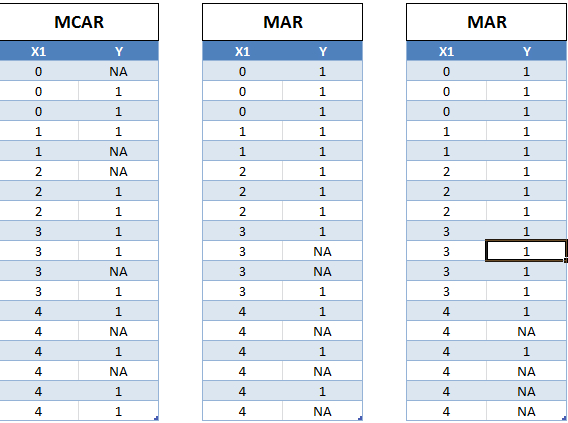
\includegraphics[width=0.55\linewidth, height=0.66\textheight]{../img/2_patterns}
		%\caption{Esquema de procesos de generación de datos perdidos}
		%\label{fig:2_patterns}
\end{figure}
\end{frame}

\begin{frame}
	\frametitle{¿Por qué es importante imputar datos?}
	\framesubtitle{Un ejemplo: EPH}
	\small{\textbf{Proporción de casos imputados (sin datos en alguna variable de ingresos) en EPH. Total de aglomerados urbanos, 2003-2018 (II-Trimestre de cada año)}}
	\begin{figure}
		\centering
		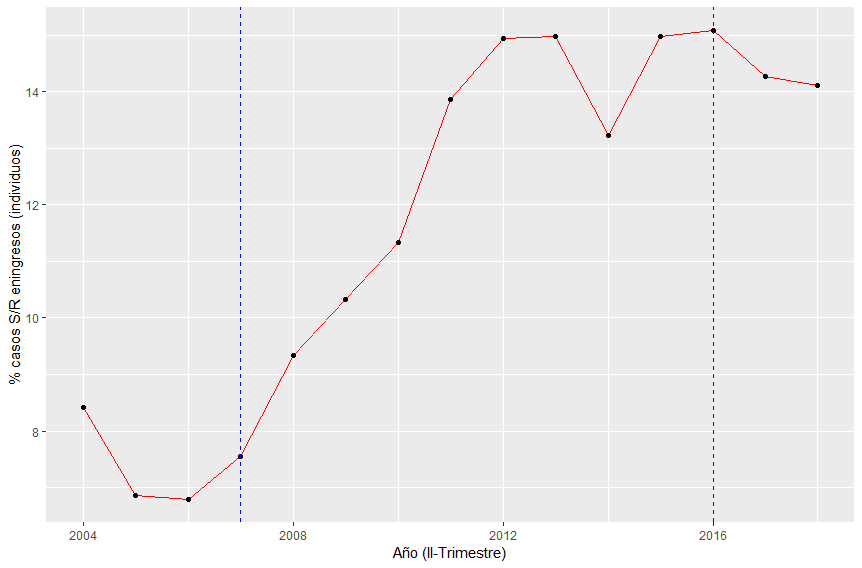
\includegraphics[width=0.7\linewidth, height=0.55\textheight]{../img/4_eph_NR2}
	\end{figure}
\end{frame}

\section{¿Cómo lidiar con valores perdidos?}
\subsection{Métodos de Imputación Simple}
\begin{frame}
	\frametitle{¿Cómo lidiar con valores perdidos?}
	\framesubtitle{Imputación simple}
		\begin{itemize}
			\item Exclusión de casos $\rightarrow$ se achica el dataset			\item Reemplazo por la media o alguna otra medida $\rightarrow$ intervalos de confianza más estrechos de forma artificial
			\item Reponderación $\rightarrow$ es incómodo trabajar con varios sets de pesos.
		\end{itemize}
\end{frame}

\begin{frame}
\frametitle{¿Cómo lidiar con valores perdidos?}
\framesubtitle{Hot Deck}
\begin{itemize}
	\item Método ampliamente usado. INDEC -hasta 2015- y Dirección de
	Estadística de la Ciudad para realizar imputaciones en EPH y EAH
	\item Reemplaza valores faltantes de un no respondente (\"receptor") con
	los valores observados de un respondente (\"donante") que es similar
	al receptor.
\end{itemize}
\end{frame}


\begin{frame}
\frametitle{¿Cómo lidiar con valores perdidos?}
\framesubtitle{Hot Deck}
\begin{itemize}
	\item \textbf{Problema 1}: selección de la métrica de similitud entre los casos
	\item \textbf{Problema 2:} selección  de los donantes. El donante es seleccionado aleatoriamente de un set de potenciales donantes hot-deck aleatorio- o bien se selecciona un solo caso donante, generalmente a partir de un algoritmo de \"vecinos cercanos" usando alguna métrica -hot-deck determinístico-.
	\end{itemize}
\end{frame}

\subsection{Técnicas de Machine Learning}
\begin{frame}
	\frametitle{¿Cómo lidiar con valores perdidos?}
	\framesubtitle{Ensamble Learning}
	\begin{columns}
		\begin{column}{0.48\textwidth}
			\begin{itemize}		
					\item Técnicas de aprendizaje supervisado donde se combinan varios modelos base.
					\item Ampliar el espacio de hipótesis posibles para mejorar la precisión predictiva del modelo combinado resultante.
					\item Los ensambles suelen ser mucho más precisos que los modelos base que los componen.
			\end{itemize}
		\end{column}
		\begin{column}{0.85\textwidth}
			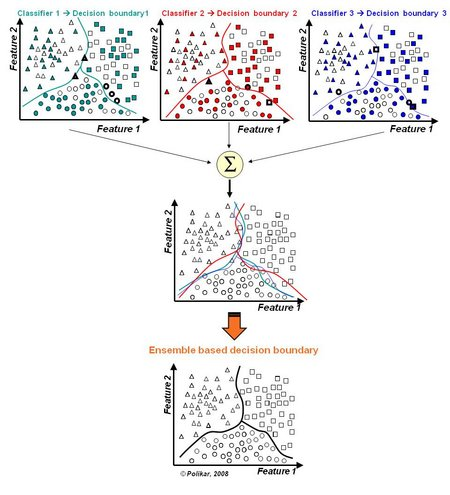
\includegraphics[width=0.657\linewidth, height=0.7\textheight]{../img/ensamble.jpg}
		\end{column}
	\end{columns}
\end{frame}

\subsubsection{Bagging}
\begin{frame}
	\frametitle{¿Cómo lidiar con valores perdidos?}
	\framesubtitle{Ensamble Learning - Bagging}
	\begin{columns}
		\begin{column}{0.48\textwidth}
	\begin{itemize}		
		\item Construcción de estimadores independientes -Boostrap-
		\item  Combinación las predicciones mediante función agregación. 
		\item Ejemplos: Random Forest, ExtraTrees, etc.
	\end{itemize}
		\end{column}
		\begin{column}{0.85\textwidth}
			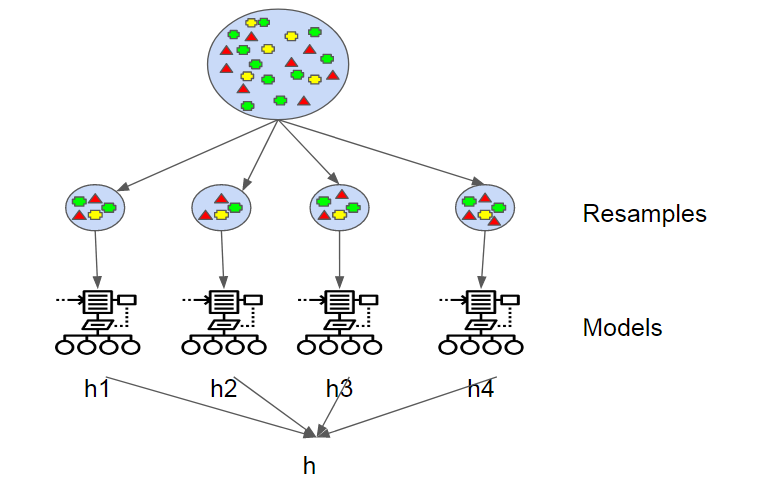
\includegraphics[width=0.7\linewidth, height=0.7\textheight]{../img/bagging}
		\end{column}
	\end{columns}
\end{frame}

\subsubsection{Boosting}
\begin{frame}
	\frametitle{¿Cómo lidiar con valores perdidos?}
	\framesubtitle{Ensamble Learning - Boosting}
	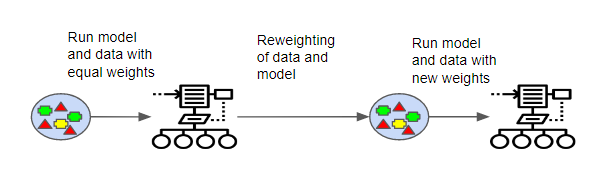
\includegraphics[width=1\linewidth, height=0.5\textheight]{../img/boosting}
	\begin{itemize}		
		\item Construcción secuencial de los estimadores 
		\item Mayor peso en aquellos casos en los que se observa una peor performance. 
		\item Ejemplos: AdaBoost y Gradient Tree Boosting, XGBoost.
	\end{itemize}
\end{frame}

\subsubsection{MLP}
\begin{frame}
\frametitle{¿Cómo lidiar con valores perdidos?}
\framesubtitle{Ensamble Learning - Multi Layer Perceptron}
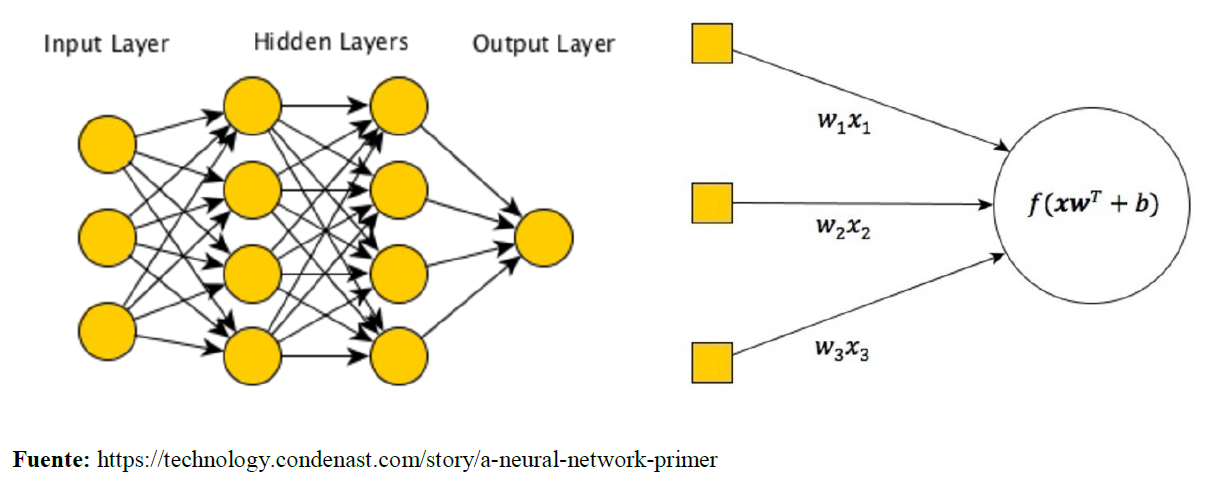
\includegraphics[width=1\linewidth, height=0.5\textheight]{../img/mlp}
\begin{itemize}		
	\item Cada neurona aplica una transformación lineal  $x_{i}w_{i}^T+b$ seguida de una función de activación
	\item Al apilar capas de neuronas se aplican sucesivas de transformaciones lineales que permiten la construcción de modelos altamente no lineales
\end{itemize}
\end{frame}

\begin{frame}
\frametitle{¿Cómo lidiar con valores perdidos?}
\framesubtitle{Ensamble Learning  - Bagging-LASSO}
\begin{figure}
	\centering
	
\includegraphics[width=0.7\linewidth]{../img/saberes}
	\label{fig:saberes}
\end{figure}
\end{frame}

\begin{frame}
\frametitle{Experimentos con EPH}
\framesubtitle{Bagging-LASSO}
\begin{itemize}
\item{Se aplica el algoritmo bagging a la imputación de ingresos laborales en la EPH del II trimestre de 2015}
\item{En cada remuestra se estima la siguiente regresión LASSO}
\begin{equation}
log_{10}(y_{i}) = \beta_{0} + \sum_{j=1}^pX_{ij}\beta_{j} + e_{i}
\end{equation}
\item{Buscando minimizar la siguiente función de costo:}
\begin{equation}
CF = RSS + \lambda\sum_{j=1}^p|\beta_{j}|
\end{equation}
\end{itemize}
\end{frame}


\subsubsection{Metodología}
\begin{frame}
\frametitle{Experimento con EPH}
\framesubtitle{Pipeline}
\begin{itemize}
	\item Dataset: EPH 2do. trimestre de 2015
	\item Población: Ocupados en la semana de referencia
	\item Variables predictoras sociodemográficas, laborales y otros ingresos
	\item Repo: \href{https://github.com/gefero/ML_imputation}{https://github.com/gefero/ML\_imputation}
\end{itemize}
\end{frame}

\begin{frame}
\frametitle{Experimento con EPH}
\framesubtitle{Pipeline}
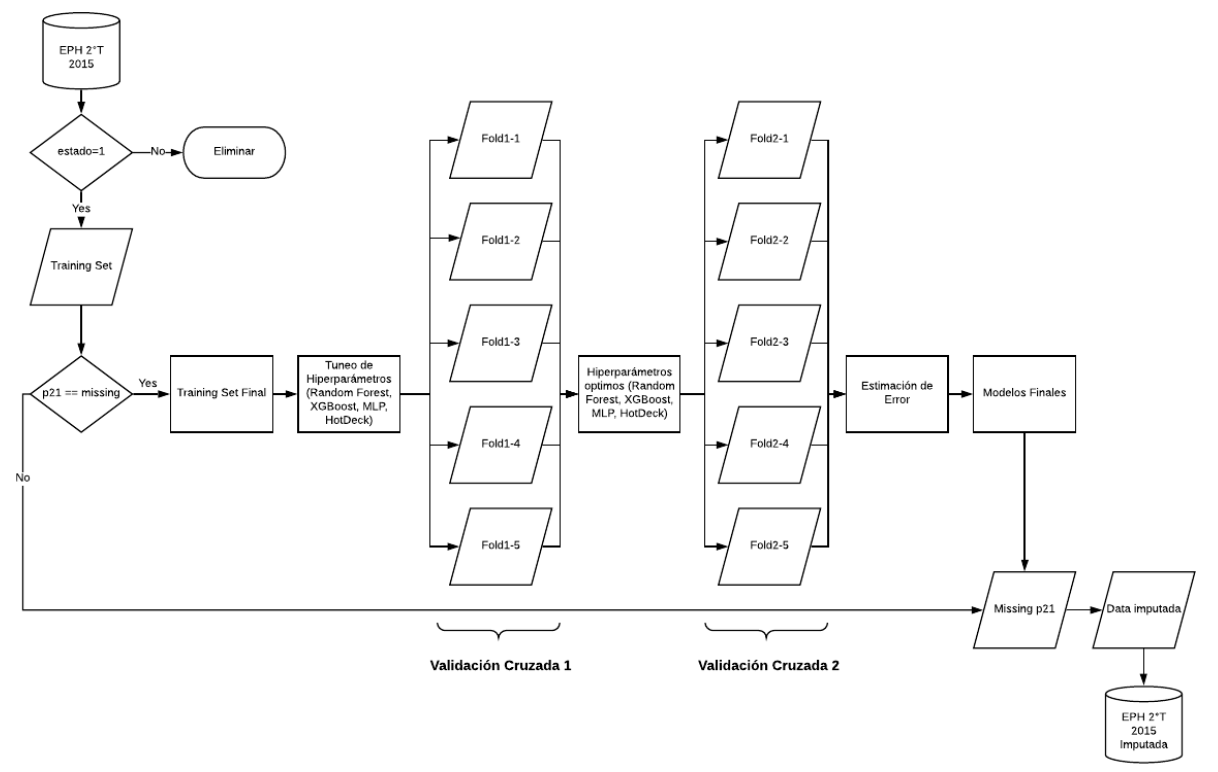
\includegraphics[width=0.99\linewidth, height=0.7\textheight]{../img/pipeline}
\end{frame}


\begin{frame}
\frametitle{Experimento con EPH}
\framesubtitle{Estrategia de validación 1}
\begin{itemize}
	\item Estimación de métricas de error
	\item Supuesto: Proceso de generación de datos perdidos MCAR o MAR
\end{itemize}
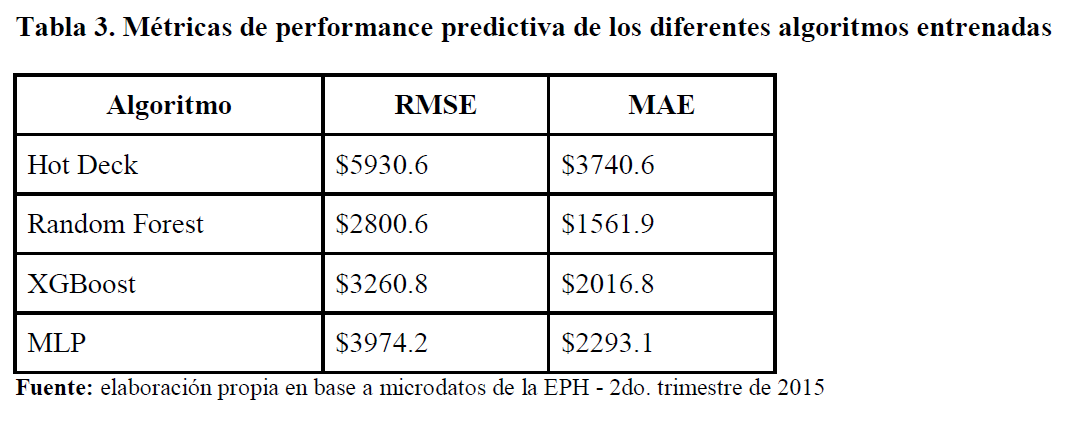
\includegraphics[width=0.85\linewidth, height=0.5\textheight]{../img/val1}
\end{frame}

\begin{frame}
\frametitle{Experimento con EPH}
\framesubtitle{Estrategia de validación 2}
Comparación de distribuciones sobre datos perdidos reales (es decir, imputados por INDEC)
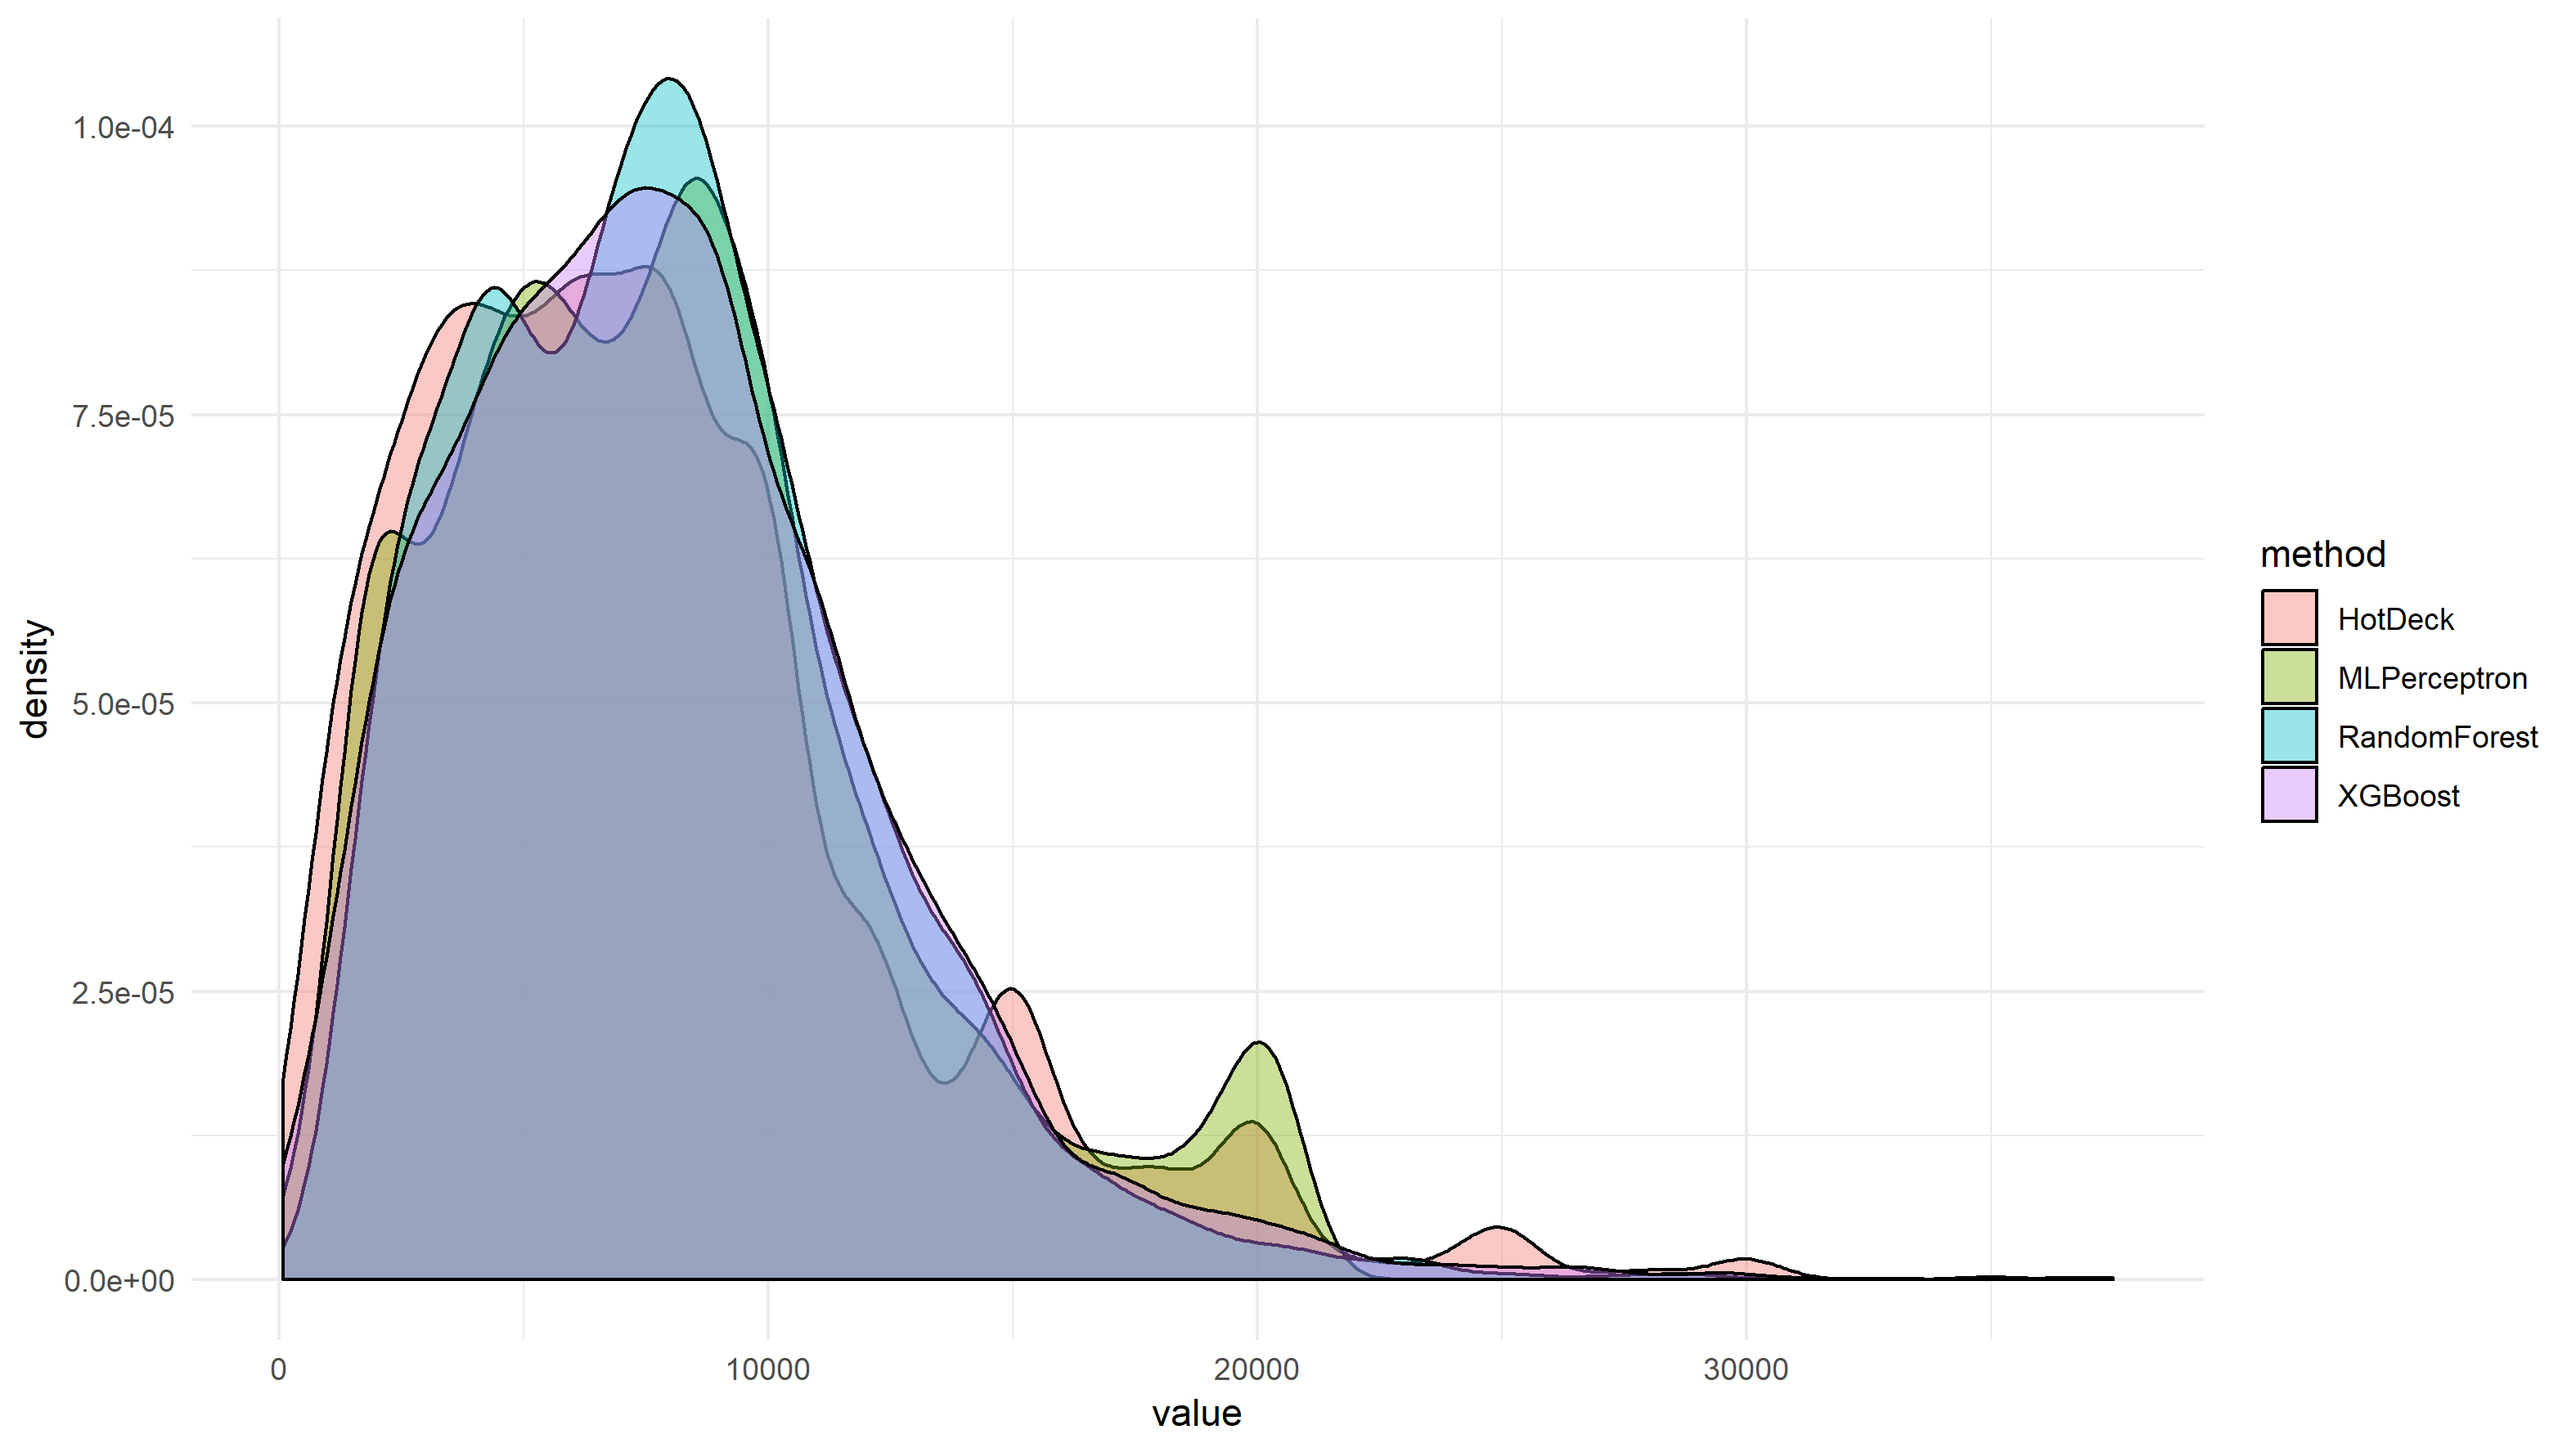
\includegraphics[width=0.85\linewidth, height=0.7\textheight]{../img/density_imp}
\end{frame}

\begin{frame}
\frametitle{Experimento con EPH}
\framesubtitle{Estrategia de validación 2}
Comparación de distribución de datos completos (imputados + respuesta)
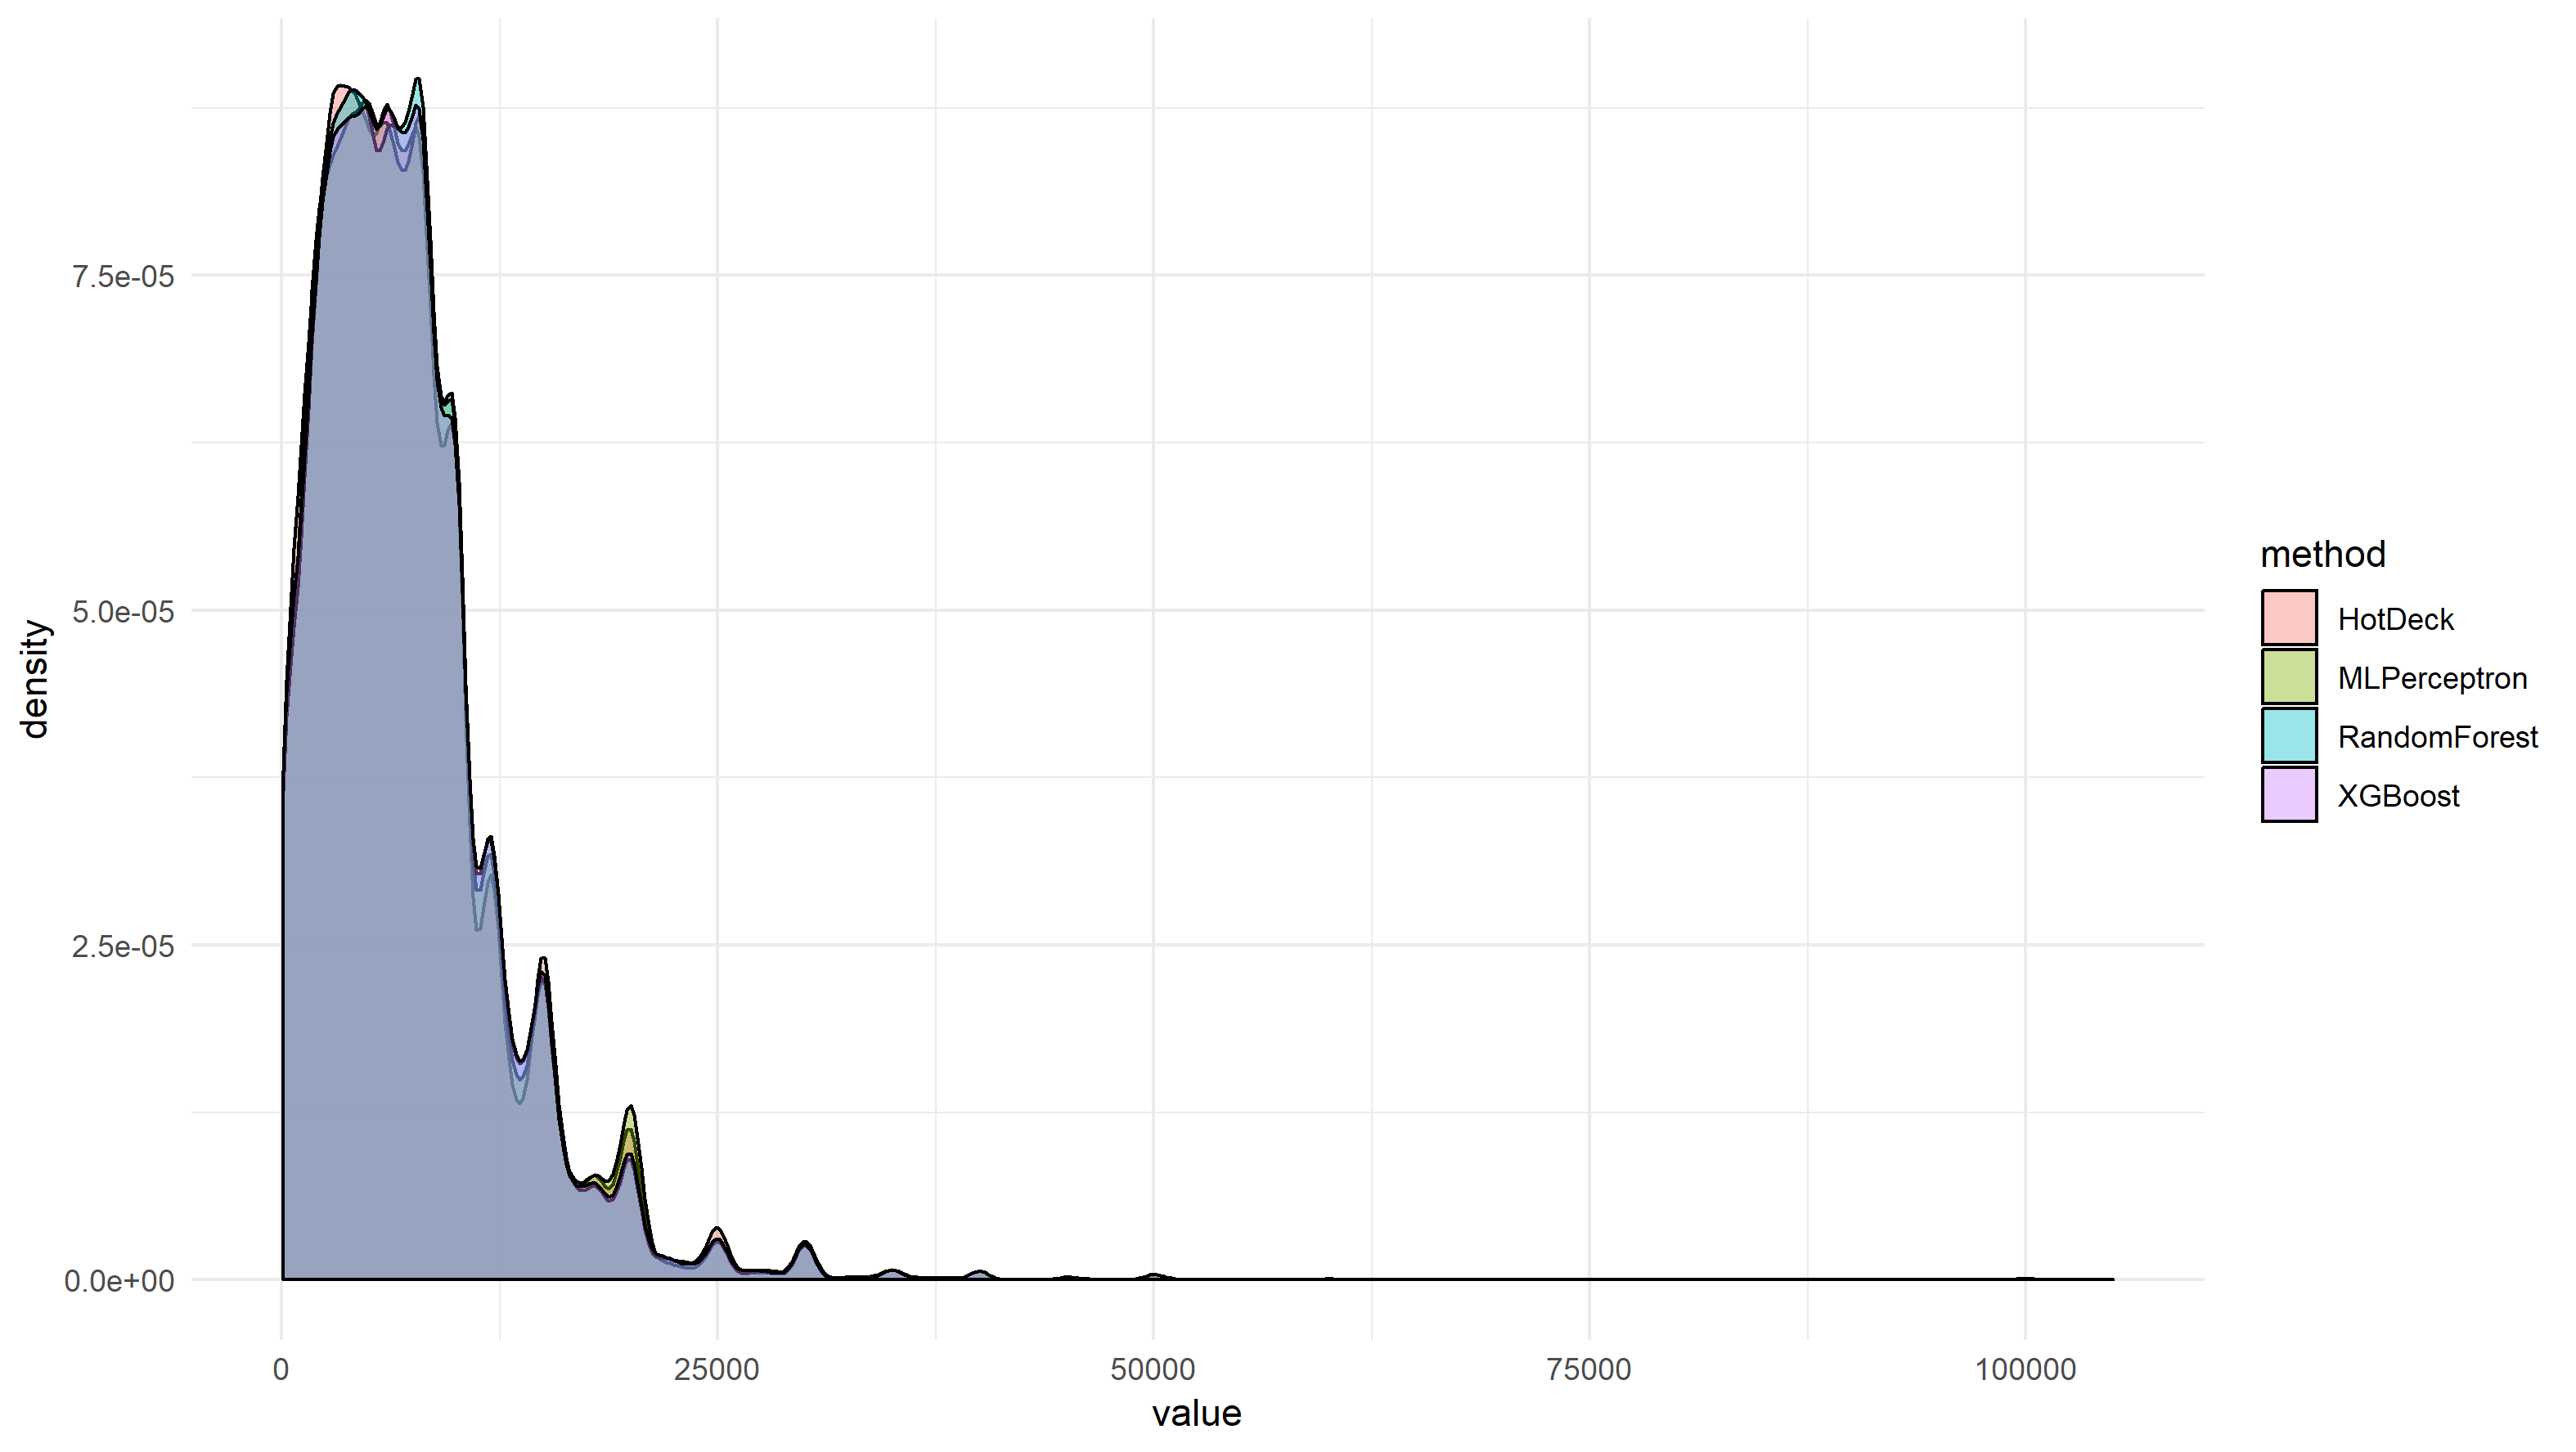
\includegraphics[width=0.85\linewidth, height=0.7\textheight]{../img/density_comp}
\end{frame}

\subsubsection{Resultados}
\begin{frame}
	\frametitle{Resumen}
	\begin{itemize}
		\item Machine Learning como alternativa para la imputación
		\item Reducción considerable en el $RMSE$ entre casos perdidos comparado a Hot Deck -entre 30\% y 50\%-
		\item Problemas a futuro
		\begin{itemize}
			\item Extensión del alcance del ejercicio
			\item Mejoras en tuneo de hiperparámetros (algoritmos de búsqueda más inteligentes, diferentes funciones de activación, etc.)
			\item Propiedades de los estimadores y estimaciones de medidas basadas en ingresos al utilizar estas técnicas
			\item Performance relativa a HotDeck en procesos de generación de datos no aleatorios
		\end{itemize}
	\end{itemize}
\end{frame}

\subsubsection{La Yapa...}
\begin{frame}
\frametitle{La Yapa... }
\framesubtitle{rindec/eph}
\begin{figure}
	\centering
	
\includegraphics[width=0.7 \linewidth, height=0.6 \textheight]{../img/rindec1}
\end{figure}
	\href{https://github.com/rindec/eph}{https://github.com/rindec/eph}
\end{frame}

\subsubsection{La Yapa...}
\begin{frame}
\frametitle{La Yapa... }
\framesubtitle{rindec/eph}
\begin{figure}
	\centering
	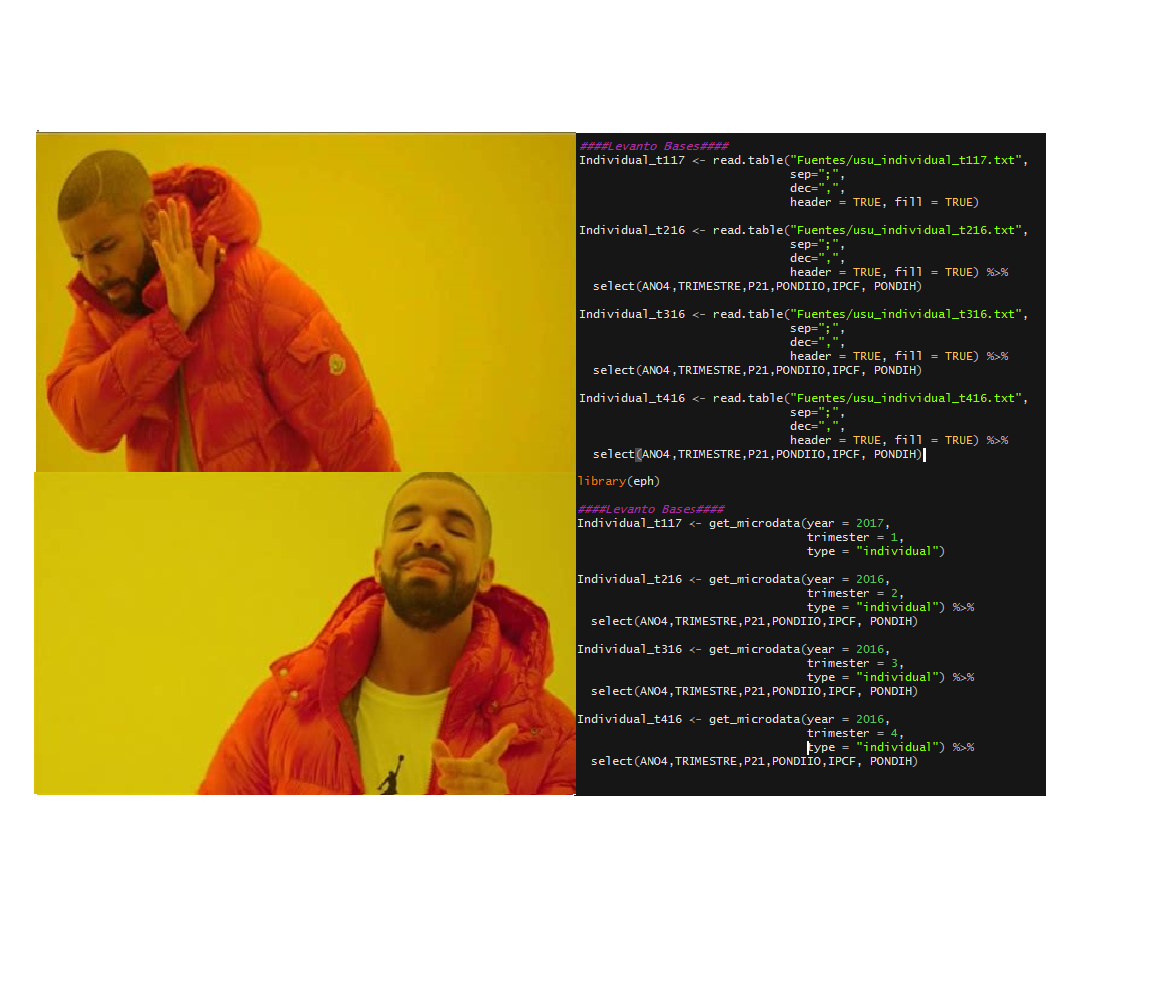
\includegraphics[width=0.8 \linewidth, height=0.7 \textheight]{../img/rindec2}
\end{figure}
\end{frame}


\begin{frame}
\frametitle{La Yapa... }
\framesubtitle{NLP - letras de tango }
\small{\textbf{Composición de tópicos de algunos tangos}}
\begin{figure}
	\centering
	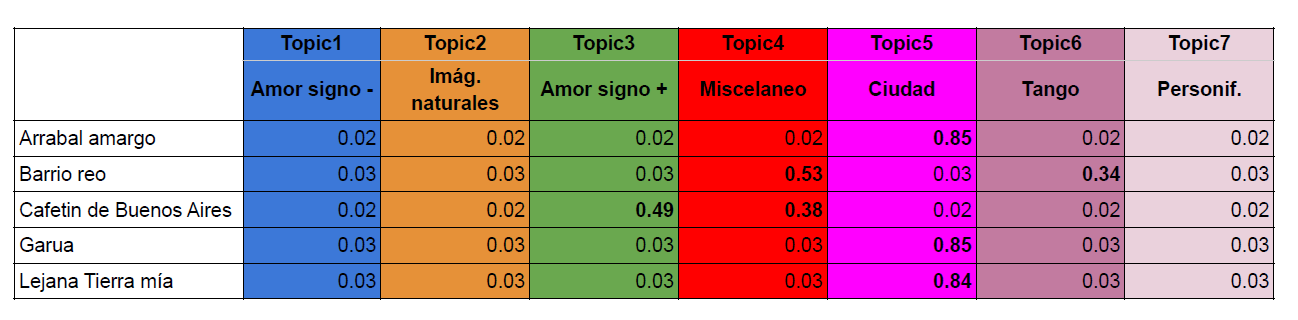
\includegraphics[width=0.9 \linewidth, height=0.35 \textheight]{../img/tango1}
\end{figure}
\end{frame}

\begin{frame}
\frametitle{La Yapa... }
\framesubtitle{NLP - letras de tango }
\small{\textbf{Evolución temporal de los tópicos}}
\begin{figure}
	\centering
	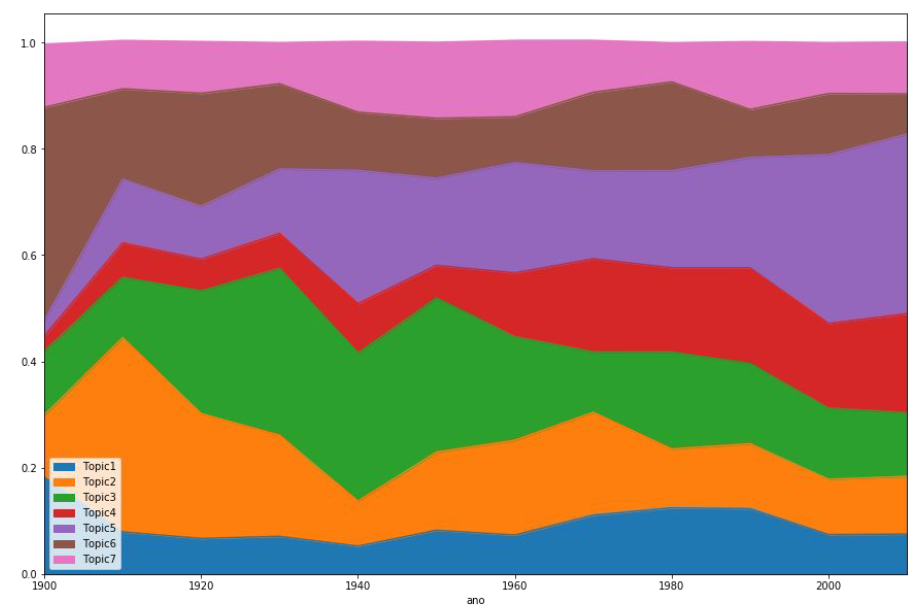
\includegraphics[width=0.9 \linewidth, height=0.7 \textheight]{../img/tango2}
\end{figure}
\end{frame}

\begin{frame}
	\begin{center}
	{\huge ¿Preguntas?
		\linebreak}
	\begin{figure}
		\centering
		
\includegraphics[width=0.7\linewidth, height=0.5\textheight]{../img/end}
		\label{fig:end}
	\end{figure}
	
	\end{center}
\end{frame}
\end{document}